\chapter{Preparation}

\section{Question 1: Open Circuit Voltage}
The Term (1)
\begin{equation}
 I_{\mathrm{PIN}} = I_{\mathrm{Sat}}\left[\exp\left(\frac{U_{\mathrm{PIN}}}{U_{\mathrm{T}}}\right)-1\right] -I_{\mathrm{pr}}
\label{eq:diode}
\end{equation}
from the experiment description, with $R_{\mathrm{a}}\to\infty(I_{\mathrm{PIN}}\to0)$ can be rearranged to:
\begin{equation}
 I_{\mathrm{pr}} = I_{\mathrm{Sat}}\left[\exp\left(\frac{U_{\mathrm{PIN0}}}{U_{\mathrm{T}}}\right)-1\right]
\end{equation}
and further to:
\begin{equation}
 U_{\mathrm{PIN0}}(I_{\mathrm{pr}}) = U_{\mathrm{T}}\ln\left(\frac{I_{\mathrm{pr}}}{I_{\mathrm{Sat}}}\right)+1
\end{equation}

\section{Question 2: Electrical Power of a PIN Diode}

With $P = R\cdot I^2$, $I_{\mathrm{pr}} = S\cdot P$ and equation \eqref{eq:diode}, the Power of the PIN-diode can be calculated by:
\begin{equation}
 P_{\mathrm{el}} = R_{\mathrm{a}}\cdot\left\{ I_{\mathrm{Sat}}\left[\exp\left(\frac{U_{\mathrm{PIN}}}{U_{\mathrm{T}}}\right)-1\right] -S\cdot P\right\}^2.
\label{eq:power}
\end{equation}
For the Case:
\begin{equation}
 \frac{U_{\mathrm{PIN}}}{U_{\mathrm{T}}} \ll 1 \to \exp\left(\frac{U_{\mathrm{PIN}}}{U_{\mathrm{T}}}\right)\approx1+\frac{U_{\mathrm{PIN}}}{U_{\mathrm{T}}}
\end{equation}
equation \eqref{eq:power} can be simplified to:
\begin{equation}
  P_{\mathrm{el}} = R_{\mathrm{a}}\cdot\left\{ I_{\mathrm{Sat}}\cdot\frac{U_{\mathrm{PIN}}}{U_{\mathrm{T}}} -S\cdot P\right\}^2.
\end{equation}
\todo{da stimmt irgendwas noch net}

\section{Question 3: Photodetector with Transimpedance Amplifier}

\begin{figure}[h]%
\centering
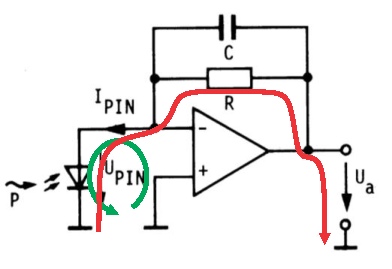
\includegraphics[width=.8\columnwidth]{Grafiken/OPAMP_m.pdf}
\caption{}%
\label{fig:OPAMP}%

\end{figure}

In Figure \ref{fig:OPAMP} with Kirchhoff's second law it can be derived (using the red loop):
\begin{equation}
 - u_{\mathrm{PIN}} - i_{\mathrm{PIN}}\cdot \frac{R}{1+ j\omega RC}+u_{\mathrm{a}} = 0 .
\label{eq:masche1}
\end{equation}
Using
\begin{equation}
 u_{\mathrm{PIN}}=0.
\label{eq:masche2}
\end{equation}
resulting also from Kirchhoff's second law (green loop) you get:
\begin{equation}
 u_{\mathrm{a}} = i_{\mathrm{PIN}}\cdot \frac{R}{1+ j\omega RC}.
\label{eq:ua}
\end{equation}

For the cut-off frequency $f_{\mathrm{3dB}}$ the following condition has to be fulfilled:
\begin{equation}
 \frac{u(f_{\mathrm{3dB}})}{u(0)} = \frac{1}{\sqrt{2}}
\end{equation}
With \eqref{eq:ua} you obtain
\begin{equation}
 \frac{i_{\mathrm{PIN}}\cdot \frac{R}{1+ j2\pi f_{\mathrm{3dB}} RC}}{i_{\mathrm{PIN}}\cdot R} = \frac{1}{\sqrt{2}}
\end{equation}
and further
\begin{equation}
 f_{\mathrm{3dB}} = \frac{\sqrt{2}-1}{j2\pi RC} 
\end{equation}

 

